\clearpage
\VerdierPhysicalPageAnchor{0092}%
\VerdierSemanticAnchor{ch1-3-2-9-eq5}
从而得到图：
\begin{equation}
  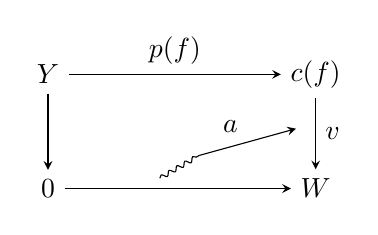
\begin{tikzpicture}[>=stealth,baseline=(current bounding box.center)]
    \node (Y)  at (0,1.45) {$Y$};
    \node (Cf) at (3.4,1.45) {$c(f)$};
    \node (Z)  at (0,0) {$0$};
    \node (W)  at (3.4,0) {$W$};
    \draw[->] (Y) -- node[above] {$p(f)$} (Cf);
    \draw[->] (Y) -- (Z);
    \draw[->] (Cf) -- node[right] {$v$} (W);
    \draw[->] (Z) -- (W);
    \draw[decorate,decoration={snake,amplitude=0.8pt,segment length=3.3pt}]
      (1.42,0.13) -- (1.92,0.42);
    \draw[->] (1.92,0.42) -- node[above left] {$a$} (3.15,0.76);
  \end{tikzpicture}
  \tag{3.2.9.5}
\end{equation}

\VerdierSemanticAnchor{ch1-3-2-9-n-morphism}
依 (3.1.3)，此图定义了与三元组
$\bigl(m\colon Y\longrightarrow W,\;a\colon0\rightsquigarrow m,\;
a\star f\colon0\rightsquigarrow mf\bigr)$ 相对应的态射
$n\colon c(p(f))\longrightarrow W$。为证明态射 $n$ 同伦于零，依 (3.1.5)，
只需证明图 (3.2.9.5) 是 $\operatorname{tr}_1(C)$ 中一个同伦于零的态射；
为此，只需证明存在同伦 $\beta\colon0\rightsquigarrow v$，使得
$\beta\star p(f)=a$。态射 $v\colon c(f)\longrightarrow W$ 的分量为：

\VerdierSemanticAnchor{ch1-3-2-9-eq6}
\begin{equation}
  v^i=(m^i,a^if^{i+1})\colon Y^i\oplus X^{i+1}\longrightarrow W^i
  \tag{3.2.9.6}
\end{equation}
而且可立即验证，分量为

\VerdierSemanticAnchor{ch1-3-2-9-eq7}
\begin{equation}
  \beta^i=(a^i,0)\colon Y^{i+1}\oplus X^{i+2}\longrightarrow W^i
  \tag{3.2.9.7}
\end{equation}

\VerdierSemanticAnchor{ch1-3-2-9-conclusion}
的同伦 $\beta$ 联结 $0$ 与 $v$，且满足 $\beta\star p(f)=a$。
这就完成了断言 (3.2.7.3) 的证明。

\VerdierSemanticAnchor{ch1-3-2-10}
\noindent\textbf{3.2.10. 断言 (3.2.7.4) 的证明。}\quad
\VerdierSemanticAnchor{ch1-3-2-10-y1-represented-functor}
对象 $Y[1]$ 表示函子：

\VerdierSemanticAnchor{ch1-3-2-10-eq1}
\begin{equation}
  W\longmapsto
  \left\{\,
  \vcenter{\hbox{%
    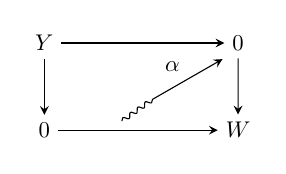
\begin{tikzpicture}[>=stealth,baseline=(current bounding box.center),scale=0.82,
      every node/.style={transform shape}]
      \node (Y) at (0,1.35) {$Y$};
      \node (ZT) at (3.0,1.35) {$0$};
      \node (ZB) at (0,0) {$0$};
      \node (W) at (3.0,0) {$W$};
      \draw[->] (Y) -- (ZT);
      \draw[->] (Y) -- (ZB);
      \draw[->] (ZT) -- (W);
      \draw[->] (ZB) -- (W);
      \draw[decorate,decoration={snake,amplitude=0.8pt,segment length=3.3pt}]
        (1.20,0.14) -- (1.68,0.48);
      \draw[->] (1.68,0.48) -- node[above left] {$\alpha$} (2.76,1.10);
    \end{tikzpicture}%
  }}\,\right\}.
  \tag{3.2.10.1}
\end{equation}

\VerdierSemanticAnchor{ch1-3-2-10-f1-functorial-map}
而态射 $f[1]\colon X[1]\longrightarrow Y[1]$ 表示函子态射：

\VerdierSemanticAnchor{ch1-3-2-10-eq2}
\begin{equation}
  \begin{gathered}
    D=
    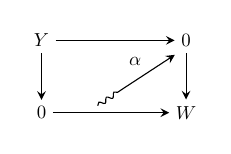
\begin{tikzpicture}[>=stealth,baseline=(current bounding box.center),scale=0.68,
      every node/.style={transform shape}]
      \node (Y) at (0,1.35) {$Y$};
      \node (ZT) at (2.7,1.35) {$0$};
      \node (ZB) at (0,0) {$0$};
      \node (W) at (2.7,0) {$W$};
      \draw[->] (Y) -- (ZT); \draw[->] (Y) -- (ZB);
      \draw[->] (ZT) -- (W); \draw[->] (ZB) -- (W);
      \draw[decorate,decoration={snake,amplitude=0.8pt,segment length=3.3pt}]
        (1.05,0.13) -- (1.48,0.42);
      \draw[->] (1.48,0.42) -- node[above left] {$\alpha$} (2.49,1.08);
    \end{tikzpicture}
    \quad\longmapsto\quad f[1]D=
    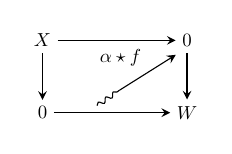
\begin{tikzpicture}[>=stealth,baseline=(current bounding box.center),scale=0.68,
      every node/.style={transform shape}]
      \node (X) at (0,1.35) {$X$};
      \node (ZT) at (2.7,1.35) {$0$};
      \node (ZB) at (0,0) {$0$};
      \node (W) at (2.7,0) {$W$};
      \draw[->] (X) -- (ZT); \draw[->] (X) -- (ZB);
      \draw[->] (ZT) -- (W); \draw[->] (ZB) -- (W);
      \draw[decorate,decoration={snake,amplitude=0.8pt,segment length=3.3pt}]
        (1.02,0.13) -- (1.44,0.42);
      \draw[->] (1.44,0.42) -- node[above left] {$\alpha\star f$} (2.49,1.08);
    \end{tikzpicture}
  \end{gathered}
  \tag{3.2.10.2}
\end{equation}
